\documentclass{ximera}
\graphicspath{  %% When looking for images,
{./}            %% look here first,
{./pictures/}   %% then look for a pictures folder,
{../pictures/}  %% which may be a directory up.
{../../pictures/}  %% which may be a directory up.
{../../../pictures/}  %% which may be a directory up.
{../../../../pictures/}  %% which may be a directory up.
}

\usepackage{listings}
%\usepackage{circuitikz}
\usepackage{xcolor}
\usepackage{amsmath,amsthm}
\usepackage{subcaption}
\usepackage{graphicx}
\usepackage{tikz}
%\usepackage{tikz-3dplot}
\usepackage{amsfonts}
%\usepackage{mdframed} % For framing content
%\usepackage{tikz-cd}

  \renewcommand{\vector}[1]{\left\langle #1\right\rangle}
  \newcommand{\arrowvec}[1]{{\overset{\rightharpoonup}{#1}}}
  \newcommand{\ro}{\texttt{R}}%% row operation
  \newcommand{\dotp}{\bullet}%% dot product
  \renewcommand{\l}{\ell}
  \let\defaultAnswerFormat\answerFormatBoxed
  \usetikzlibrary{calc,bending}
  \tikzset{>=stealth}
  




%make a maroon color
\definecolor{maroon}{RGB}{128,0,0}
%make a dark blue color
\definecolor{darkblue}{RGB}{0,0,139}
%define the color fourier0 to be the maroon color
\definecolor{fourier0}{RGB}{128,0,0}
%define the color fourier1 to be the dark blue color
\definecolor{fourier1}{RGB}{0,0,139}
%define the color fourier 1t to be the light blue color
\definecolor{fourier1t}{RGB}{173,216,230}
%define the color fourier2 to be the dark green color
\definecolor{fourier2}{RGB}{0,100,0}
%define teh color fourier2t to be the light green color
\definecolor{fourier2t}{RGB}{144,238,144}
%define the color fourier3 to be the dark purple color
\definecolor{fourier3}{RGB}{128,0,128}
%define the color fourier3t to be the light purple color
\definecolor{fourier3t}{RGB}{221,160,221}
%define the color fourier0t to be the red color
\definecolor{fourier0t}{RGB}{255,0,0}
%define the color fourier4 to be the orange color
\definecolor{fourier4}{RGB}{255,165,0}
%define the color fourier4t to be the darker orange color
\definecolor{fourier4t}{RGB}{255,215,0}
%define the color fourier5 to be the yellow color
\definecolor{fourier5}{RGB}{255,255,0}
%define the color fourier5t to be the darker yellow color
\definecolor{fourier5t}{RGB}{255,255,100}
%define the color fourier6 to be the green color
\definecolor{fourier6}{RGB}{0,128,0}
%define the color fourier6t to be the darker green color
\definecolor{fourier6t}{RGB}{0,255,0}

%New commands for this doc for errors in copying
\newcommand{\eigenvar}{\lambda}
%\newcommand{\vect}[1]{\mathbf{#1}}
\renewcommand{\th}{^{\text{th}}}
\newcommand{\st}{^{\text{st}}}
\newcommand{\nd}{^{\text{nd}}}
\newcommand{\rd}{^{\text{rd}}}
\newcommand{\paren}[1]{\left(#1\right)}
\newcommand{\abs}[1]{\left|#1\right|}
\newcommand{\R}{\mathbb{R}}
\newcommand{\C}{\mathbb{C}}
\newcommand{\Hilb}{\mathbb{H}}
\newcommand{\qq}[1]{\text{#1}}
\newcommand{\Z}{\mathbb{Z}}
\newcommand{\N}{\mathbb{N}}
\newcommand{\q}[1]{\text{``#1''}}
%\newcommand{\mat}[1]{\begin{bmatrix}#1\end{bmatrix}}
\newcommand{\rref}{\text{reduced row echelon form}}
\newcommand{\ef}{\text{echelon form}}
\newcommand{\ohm}{\Omega}
\newcommand{\volt}{\text{V}}
\newcommand{\amp}{\text{A}}
\newcommand{\Seq}{\textbf{Seq}}
\newcommand{\Poly}{\textbf{P}}
\renewcommand{\quad}{\text{    }}
\newcommand{\roweq}{\simeq}
\newcommand{\rowop}{\simeq}
\newcommand{\rowswap}{\leftrightarrow}
\newcommand{\Mat}{\textbf{M}}
\newcommand{\Func}{\textbf{Func}}
\newcommand{\Hw}{\textbf{Hamming weight}}
\newcommand{\Hd}{\textbf{Hamming distance}}
\newcommand{\rank}{\text{rank}}
\newcommand{\longvect}[1]{\overrightarrow{#1}}
% Define the circled command
\newcommand{\circled}[1]{%
  \tikz[baseline=(char.base)]{
    \node[shape=circle,draw,inner sep=2pt,red,fill=red!20,text=black] (char) {#1};}%
}

% Define custom command \strikeh that just puts red text on the 2nd argument
\newcommand{\strikeh}[2]{\textcolor{red}{#2}}

% Define custom command \strikev that just puts red text on the 2nd argument
\newcommand{\strikev}[2]{\textcolor{red}{#2}}

%more new commands for this doc for errors in copying
\newcommand{\SI}{\text{SI}}
\newcommand{\kg}{\text{kg}}
\newcommand{\m}{\text{m}}
\newcommand{\s}{\text{s}}
\newcommand{\norm}[1]{\left\|#1\right\|}
\newcommand{\col}{\text{col}}
\newcommand{\sspan}{\text{span}}
\newcommand{\proj}{\text{proj}}
\newcommand{\set}[1]{\left\{#1\right\}}
\newcommand{\degC}{^\circ\text{C}}
\newcommand{\centroid}[1]{\overline{#1}}
\newcommand{\dotprod}{\boldsymbol{\cdot}}
%\newcommand{\coord}[1]{\begin{bmatrix}#1\end{bmatrix}}
\newcommand{\iprod}[1]{\langle #1 \rangle}
\newcommand{\adjoint}{^{*}}
\newcommand{\conjugate}[1]{\overline{#1}}
\newcommand{\eigenvarA}{\lambda}
\newcommand{\eigenvarB}{\mu}
\newcommand{\orth}{\perp}
\newcommand{\bigbracket}[1]{\left[#1\right]}
\newcommand{\textiff}{\text{ if and only if }}
\newcommand{\adj}{\text{adj}}
\newcommand{\ijth}{\emph{ij}^\text{th}}
\newcommand{\minor}[2]{M_{#2}}
\newcommand{\cofactor}{\text{C}}
\newcommand{\shift}{\textbf{shift}}
\newcommand{\startmat}[1]{
  \left[\begin{array}{#1}
}
\newcommand{\stopmat}{\end{array}\right]}
%a command to give a name to explorations and hints and theorems
\newcommand{\name}[1]{\begin{centering}\textbf{#1}\end{centering}}
\newcommand{\vect}[1]{\vec{#1}}
\newcommand{\dfn}[1]{\textbf{#1}}
\newcommand{\transpose}{\mathsf{T}}
\newcommand{\mtlb}[2][black]{\texttt{\textcolor{#1}{#2}}}
\newcommand{\RR}{\mathbb{R}} % Real numbers
\newcommand{\id}{\text{id}}
\newcommand{\coord}[1]{\langle#1\rangle}
\newcommand{\RREF}{\text{RREF}}
\newcommand{\Null}{\text{Null}}
\newcommand{\Nullity}{\text{Nullity}}
\newcommand{\Rank}{\text{Rank}}
\newcommand{\Col}{\text{Col}}
\newcommand{\Ef}{\text{EF}}
\newcommand{\boxprod}[3]{\abs{(#1\times#2)\cdot#3}}

\author{Zack Reed}
%borrowed from ximera interactive la
\title{Determinants in Higher Dimensions}
\begin{document}
\begin{abstract}

\end{abstract}
\maketitle

\section*{Interpreting the Sign of the Determinant}

The sign of an integral tells us the relative height orientation of a function's graph to the $x$-axis. 

\begin{example}
    
Consider the function $f(x)=\cos(x)$ between $\pi/2$ and $3\pi/2$.

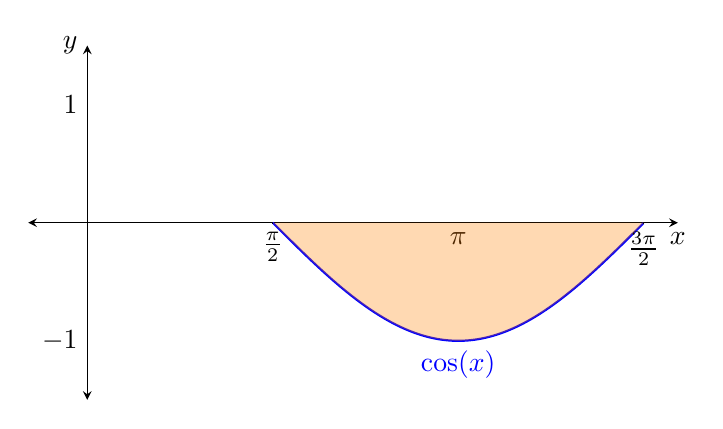
\begin{tikzpicture}[scale=1.5]
    % Draw axes
    \draw[<->] (-0.5,0) -- (5,0) node[below] {\(x\)};
    \draw[<->] (0,-1.5) -- (0,1.5) node[left] {\(y\)};
    
    % Draw the cosine function
    \draw[thick,blue,samples=100,domain=1.57:4.71] 
        plot (\x,{cos(\x r)}); %node[right] {\(\cos(x)\)};
    
    \node[anchor=north, blue] at (3.14,-1) {\(\cos(x)\)};
    %\node[anchor=north, blue] at (3.14,-1) {\(cos(x)\)};
    
    % Label important points on the x-axis
    \node[below] at (1.57,0) {\(\frac{\pi}{2}\)};
    \node[below] at (3.14,0) {\(\pi\)};
    \node[below] at (4.71,0) {\(\frac{3\pi}{2}\)};
    
    % Add dashed lines for bounds
    \draw[dashed] (1.57,0) -- (1.57,{cos(1.57 r)});
    \draw[dashed] (4.71,0) -- (4.71,{cos(4.71 r)});

    % Shade the area under the curve
    \begin{scope}
        \clip (1.57,-1.5) rectangle (4.71,1.5); % Clip the shading to the bounds
        \fill[orange,opacity=0.3] plot[smooth,samples=100,domain=1.57:4.71] (\x,{cos(\x r)}) -- (4.71,0) -- (1.57,0) -- cycle;
    \end{scope}
    
    % Label y-axis
    \node[left] at (0,1) {\(1\)};
    \node[left] at (0,-1) {\(-1\)};
\end{tikzpicture}

The integral $\int_{\pi/2}^{3\pi/2}\cos(x)\cdot\ dx=-2$. We know that the area measure here is $\answer{2}$ units, but the $-$ sign tells us that the region is located \wordChoice{\choice{above}\choice[correct]{below}} the $x$-axis.

\end{example}

Similarly, the sign of the determinant tells us information about relative orientation. Though fundamentally they are connected, we are not measuring relative orientation to an axis, but relative orientation of the transformed unit vectors. 

\begin{example}
    Utilizing the following GeoGebra applet, explore the transformed area measure for the following matrices, attending to the relative orientation of the unit vectors under the transformation.

    Specifically, if we consider the ``order'' of the unit vectors $\vec{i}$ and $\vec{j}$, we tend to put $\vec{i}$ before $\vec{j}$. 


    \begin{center}
        \geogebra{uc5xg9qj}{549}{388}
    \end{center}
    
    From a perspective of relative orientation in space,we might colloquially say $\vec{i}$ is ``before'' $\vec{j}$ in the sense that rotating from $\vec{i}$ to $\vec{j}$ creates an angle measure less than $180^\circ$.

    So, the identity matrix $I=\begin{bmatrix}
        1&0\\0&1
    \end{bmatrix}$, encodes a transformation of preserving the original area of space, and preserving the relative orientation of the unit vectors. 

    In the applet, alter the matrix so that it changes the order of the unit vectors, and view the resulting determinant:

    In the matrix $A=\begin{bmatrix}
        0&1\\1&0
    \end{bmatrix}$, the vector $\vec{i}$ is \wordChoice{
        \choice{before}
        \choice[correct]{after}
    }
    the vector $\vec{j}$, and the determinant is $\answer{-1}$.

    This is an example of the information gained by the sign of the determinant.

\end{example}

Let's do some more examples to further illustrate this phenomenon. 

\begin{example}
    For the following matrices, determine the amount of stretching or compressing of the transformation, and the relative orientation of the unit vectors $\vec{i}$ and $\vec{j}$. 

    \begin{enumerate}
        \item The rotation matrix $R=\begin{bmatrix}
            \cos(\pi/4)& -\sin(\pi/4)\\ \sin(\pi/4) & \cos(\pi/4)
        \end{bmatrix}$ scales spatial area by a (positive) measure of $\answer{1}$ and from a relative orientation perspective (as described in the last example) the transformed unit vector $A\vec{i}$ is \wordChoice{
            \choice[correct]{before}
            \choice{after}
        } $A\vec{j}$.
        \item The scaling matrix $S=\begin{bmatrix}
            4& 0\\ 0 & -3
        \end{bmatrix}$ scales spatial area by a (positive) measure of $\answer{12}$ and from a relative orientation perspective (as described in the last example) the transformed unit vector $A\vec{i}$ is \wordChoice{
            \choice{before}
            \choice[correct]{after}
        } $A\vec{j}$.
        \item The matrix $A=\begin{bmatrix}
            -2& 4\\ 3 & -3
        \end{bmatrix}$ scales spatial area by a (positive) measure of $\answer{6}$ and from a relative orientation perspective (as described in the last example) the transformed unit vector $A\vec{i}$ is \wordChoice{
            \choice{before}
            \choice[correct]{after}
        } $A\vec{j}$.
        \item The matrix $B=\begin{bmatrix}
            4& -4\\ 4 & 0
        \end{bmatrix}$ scales spatial area by a measure of $\answer{16}$ and from a relative orientation perspective (as described in the last example) the transformed unit vector $A\vec{i}$ is \wordChoice{
            \choice[correct]{before}
            \choice{after}
        } $A\vec{j}$.
    \end{enumerate}
\end{example}

As we upscale the determinant to higher dimensions, these are the primary properties that we want to maintain:

\begin{enumerate}
    \item The determinant should give a measure of the transformed `volume' of space (e.g. area ($2D$), volume ($3D$), hypervolume (higher dimension)).
    \item The determinant should give some indication of the relative re-ordering of unit vectors under the transformation.
\end{enumerate}

The second point will still rely on the sign of the determinant, but it will tell us whether an odd number of unit vectors were re-ordered (negative sign) or an even number of unit vectors were re-ordered (positive sign).


\section*{The Determinant in Higher Dimensions}

We will give the general idea of how the determinant is calculated in higher dimensions, but will not dwell on this method and will instead rely on technology to compute determinants for us. 

Having a rough idea of possible algorithms but not being concerned with the details should be your main goal for this section.

\subsection*{The Determinant in 3D}

$3D$ determinants will provide us with simple examples of the method of \emph{expansion by minors}, which is how determinants can be calculated for higher dimensions, though we will not dwell on this method.

The main idea is to algorithmically break down the determinant calculations into many $2\times 2$ determinant calculations so that we acheive the goals for the determinant discussed in the previous section. This is achieved by creating multiple determinant calculations on a column-by-column (or row-by-row) basis. 

Take the $3\times 3$ matrix 

$$A=\begin{bmatrix}a&b&c\\d&e&f\\g&h&i\end{bmatrix}.$$

We expand along the top row, forming three ``\emph{entry}-\emph{minor}'' pairings, where the entry is the row-column entry of the matrix (e.g. $a$, $b$, $c$) and the ``minor'' is the rest of the matrix except for the rest of the entry's column. 

See the following entry-minor pairings for $A$:

\begin{enumerate}
    \item First, we pair the entry $a$ with the $2\times 2$ matrix $\begin{bmatrix}
        e&f\\i&h
    \end{bmatrix}$, from excluding the matrix entries in the row and column of $a$

    $$
    \begin{bmatrix}
    a & \textcolor{red}{\cancel{b}} & \textcolor{red}{\cancel{c}} \\
    \textcolor{red}{\cancel{d}} & e & f \\
    \textcolor{red}{\cancel{g}} & h & i
    \end{bmatrix}
    $$

    \item Then, we pair the entry $b$ with the $2\times 2$ matrix $\begin{bmatrix}
        d&f\\g&h
    \end{bmatrix}$, from excluding the matrix entries in the row and column of $a$

    $$
    \begin{bmatrix}
    \textcolor{red}{\cancel{a}} & b & \textcolor{red}{\cancel{c}} \\
    d & \textcolor{red}{\cancel{e}} & f \\
    g & \textcolor{red}{\cancel{i}} & h
    \end{bmatrix}
    $$

    \item Finally, we pair the entry $c$ with the $2\times 2$ matrix $\begin{bmatrix}
        d&e\\g&i
    \end{bmatrix}$, from excluding the matrix entries in the row and column of $a$

    $$
    \begin{bmatrix}
    \textcolor{red}{\cancel{a}} & \textcolor{red}{\cancel{b}} & c \\
    d & e & \textcolor{red}{\cancel{f}} \\
    g & h & \textcolor{red}{\cancel{i}}
    \end{bmatrix}
    $$

\end{enumerate}

With these three entry-minor pairs, we then multiply the entry and the determinant of the minor. So we get the three products

$a\cdot\mbox{det}\left(\begin{bmatrix}
    e&f\\i&h
\end{bmatrix}\right)$, $b\cdot \mbox{det}\left(\begin{bmatrix}
    d&f\\g&i
\end{bmatrix}\right)$, and $c\cdot \mbox{det}\left(\begin{bmatrix}
    d&e\\g&h
\end{bmatrix}\right)$.

To then preserve the orientation-ordering of the matrix, we subtract the $b$-pairing and add the others to make a final sum 

$$\mbox{det}(A)=a\cdot\mbox{det}\left(\begin{bmatrix}
    e&f\\i&h
\end{bmatrix}\right)-b\cdot \mbox{det}\left(\begin{bmatrix}
    d&f\\g&i
\end{bmatrix}\right)+c\cdot \mbox{det}\left(\begin{bmatrix}
    d&e\\g&h
\end{bmatrix}\right).$$

There are many linear algebra books that go over the process of finding the determinant more formally, including the texts referenced in the \href{https://ximera.osu.edu/appliedlinearalgebra/a1Copyright/learningActivities/m0Copyright/textHistory}{Text History} (Link) page at the beginning of this text.

\begin{example}
    Using the GeoGebra applet that follows, verify that this expansion-by-minors algorithm does compute the transformed volume of the matrix 
    
    $$A=\begin{bmatrix}
        1&2&3\\-1&1&2\\1&1&0
    \end{bmatrix}.$$

    \begin{center}
        \geogebra{mdes5d4h}{858}{509}
    \end{center}

    Remember that the applet has you enter the columns as row vectors. 

    Expansion by minors (in the order of the entries in the top row) yields the three calculations $\answer{1}\cdot\mbox{det}\left(\begin{bmatrix}
        \answer{1} & \answer{2}\\\answer{1}&\answer{0}
    \end{bmatrix}\right)$, $\answer{2}\cdot\mbox{det}\left(\begin{bmatrix}
        \answer{-1} & \answer{2}\\\answer{1}&\answer{0}
    \end{bmatrix}\right)$, and $\answer{3}\cdot\mbox{det}\left(\begin{bmatrix}
        \answer{-1} & \answer{1}\\\answer{1}&\answer{1}
    \end{bmatrix}\right)$.

    Putting these determinants and products together yields

    $$\mbox{det}(A)=\answer{-2}-\answer{-4}+\answer{-6}=\answer{-4}.$$

    The final result should match the transformed volume in the applet.
\end{example}

As you can see, this process is tedious by hand, so from here on out we will use technology to calculate the determinant for us. The command in MATLAB is $\texttt{det(A)}$, where $A$ is the defined matrix. 

\section*{Properties of the Determinant}

Here are some nice properties of the determinant. Specifically, these let you find the determinant of a matrix that is constructed in relation to other known matrices. These are true for determinants of $n\times n$ matrices of any size. 

As an example, if you know $\mbox{det}(A)=a$ and $\mbox{det}(B)=b$ for $n\times n$ matrices $A$ and $B$, you immediately know $\mbox{det}(A*B)=a\cdot b$. The following similar results help us make various quick calculations with determinants, and will be useful on the homework and moving forward. These results are not proven in this text, but the proofs can be found in any of the listed texts in the \href{https://ximera.osu.edu/appliedlinearalgebra/a1Copyright/learningActivities/m0Copyright/textHistory}{Text History} (Link) page at the beginning of this text.

\begin{theorem}
    The following properties hold true of the determinant for any matrices of size $n\times n$.
    \begin{enumerate}
        \item $\mbox{det}(I)=1$, where $I$ is the identity matrix.
        \item If $\mbox{det}(A)=a$ and $\mbox{det}(B)=b$ for $n\times n$ matrices $A$ and $B$, then $\mbox{det}(A*B)=a\cdot b$.
        \item If $A$ is invertible, then $\mbox{det}(A^{-1})=\frac{1}{\mbox{det}(A)}$.
        \item If you make matrix $A'$ by swapping two rows (or two columns) of a matrix $A$, then $\mbox{det}(A')=-\mbox{det}(A)$. In other words, swapping two rows (or columns) of a matrix negates the determinant of the original matrix. 
        \item If you make matrix $A'$ by multiplying a row of matrix $A$ by a constant $t$, then $\mbox{det}(A')=t\cdot \mbox{det}(A)$. In other words, scaling a row of a matrix also scales the determinant.
        \item The determinant of a triangular matrix is the product of the diagonal entries (i.e. the pivots).
        \item $\mbox{det}(A)=0$ if and only if $A$ is not invertible.
        \item $\mbox{det}(A^T)=\mbox{det}(A)$.
    \end{enumerate}
\end{theorem}

\subsection*{Higher Dimensions}

In higher dimensions, the process of minor expansion is the same, but the determinants cascade. For instance, in a $4\times 4$ matrix, the first minor expansion across the top row yields four entry-minor pairs, but the minors are $3\times 3$ matrices, so the minor determinants each require further expansion by minors, yielding $12$ calculations overall, plus the final summation and tracking of when to add and subtract to preserve the relative coordinate vector orientations.

Here is a general representation of one minor expansion in a general matrix:

$$
\begin{bmatrix}
    \textcolor{red}{\cancel{a_{1,1}}} & \textcolor{red}{\cancel{a_{1,2}}} & \ldots & \textcolor{red}{\cancel{a_{1,k-1}}} & a_{1,k} & \textcolor{red}{\cancel{a_{1,k+1}}} & \ldots & \textcolor{red}{\cancel{a_{1,n}}} \\
    a_{2,1} & a_{2,2} & \ldots & a_{2,k-1} & \textcolor{red}{\cancel{a_{2,k}}} & a_{2,k+1} & \ldots & a_{2,n} \\
    a_{3,1} & a_{3,2} & \ldots & a_{3,k-1} & \textcolor{red}{\cancel{a_{3,k}}} & a_{3,k+1} & \ldots & a_{3,n} \\
    \vdots & \vdots & \ddots & \vdots & \vdots & \vdots & \ddots & \vdots \\
    a_{n,1} & a_{n,2} & \ldots & a_{n,k-1} & \textcolor{red}{\cancel{a_{n,k}}} & a_{n,k+1} & \ldots & a_{n,n} \\
\end{bmatrix}
$$

If we undertake the task of finding the determinant of this matrix, for each column we do a minor expansion such as represented above. In each $k$-th column, you get the entry in the top row $a_{1,k}$ and then the minor matrix from the sub-matrix excluding the top row and the $k$-th column. This portion of the determinant is then the product

$$a_{1,k}\cdot\mbox{det}\left(
\begin{bmatrix}
    a_{2,1} & a_{2,2} & \ldots & a_{2,k-1} & a_{2,k+1} & \ldots & a_{2,n} \\
    a_{3,1} & a_{3,2} & \ldots & a_{3,k-1} & a_{3,k+1} & \ldots & a_{3,n} \\
    \vdots & \vdots & \ddots & \vdots & \vdots  & \ddots & \vdots \\
    a_{n,1} & a_{n,2} & \ldots & a_{n,k-1} & a_{n,k+1} & \ldots & a_{n,n} \\
\end{bmatrix}
\right).$$

You then do this for each entry in the first row, and then proceed in a similar fashion for each subsequent minor matrix until the process reduces to $2\times 2$ matrices. 

There are various numerical ways of speeding up this algorithm, but this is the formal construction that preserves the two important properties of the determinant: 1) the measuring of volume for the transformation, and 2) the use of the determinant sign to convey whether an even or odd number of unit vectors have changed relative orientation. 



\end{document}

